\chapter{Literature Review}
\phantomsection
\label{ch:literature}

\section{Overview}
\phantomsection
\label{sec:ocr-overview}
This chapter provides a comprehensive literature review covering several 
key aspects of Optical Character Recognition (OCR). 
It begins with a definition of OCR, followed by an overview of its technological
 evolution over time. Particular attention is given to the unique challenges 
 associated with Khmer OCR, a low-resource language with complex script characteristics.
  The chapter also explores the significant role of synthetic data in addressing data 
  scarcity for low-resource language processing and dataset development.
   Finally, the chapter concludes by identifying and summarizing the existing 
   research gaps in the current literature, highlighting areas that remain 
   under-explored and underscoring the need for further investigation.


\section{Definition of Optical Character Recognition (OCR)}
\phantomsection
\label{sec:ocr-definition}
Optical Character Recognition (OCR) is a field of computer vision and pattern recognition
 that focuses on the automatic identification and digitization of printed or handwritten 
 text from images, scanned documents, or other visual media \cite{singh2012survey}. 
 OCR systems aim to convert visual representations of text into machine-encoded formats, 
 enabling automated indexing, editing, and data extraction \cite{muaz2015khmerocr}.

Modern OCR technology has evolved significantly from its early rule-based and template-matching
roots to incorporate advanced machine learning techniques, particularly deep learning,
which allow for improved accuracy in character detection, segmentation, and classification across 
diverse languages and scripts.

OCR systems typically consist of several key components: image preprocessing (e.g., noise removal, binarization), text detection, character segmentation, feature extraction, and recognition. These systems must be adapted to handle various font styles, image distortions, complex layouts, and script-specific features. While OCR for Latin-based languages has become highly accurate, extending such systems to non-Latin scripts—such as Khmer—remains a significant research challenge due to unique linguistic and structural characteristics.
   
\section{Evolution of OCR Technology}
\phantomsection
\label{sec:synthetic-data}
Nowadays, optical character recognition (OCR), plays an instrumental role in extracting text from images,
scanned documents, and other visual media. pattern recognition technology took shape almost 100 years ago.
Many iterations later, it evolved into optical character recognition (OCR) systems solutions that are
now being used.

Fast-forwarding to the present, this technology is used by organizations to digitize their documents, because
of they want to convert unstructured data into structured data such as document, PDFs, and images into
machine-readable text.

In this section, we cover the history of OCR technology: how it began, 
how it has changed through time, and its current state.

\subsection{Early Concepts (1920s-1930s)}
\phantomsection
OCR technology has ties to telegraphy. Around the time of the First World War, 
typewriters and telegraphs were already in use. Physicist Emanuel Goldberg invented a
machine that could read characters and convert them into telegraph code. 

In the 1920s, he went further and created the first electronic document retrieval system. 
While businesses were microfilming financial records at that time, retrieving specific 
records from films was still impossible. To overcome this shortcoming, Goldberg used a 
photoelectric cell for pattern recognition using a movie projector, and this machine was 
called “The Statistical Machine.”  

The machine could sort mail and decipher bank checks through patterns that were unseen by the human eye. 

\begin{figure}[ht]
    \centering
    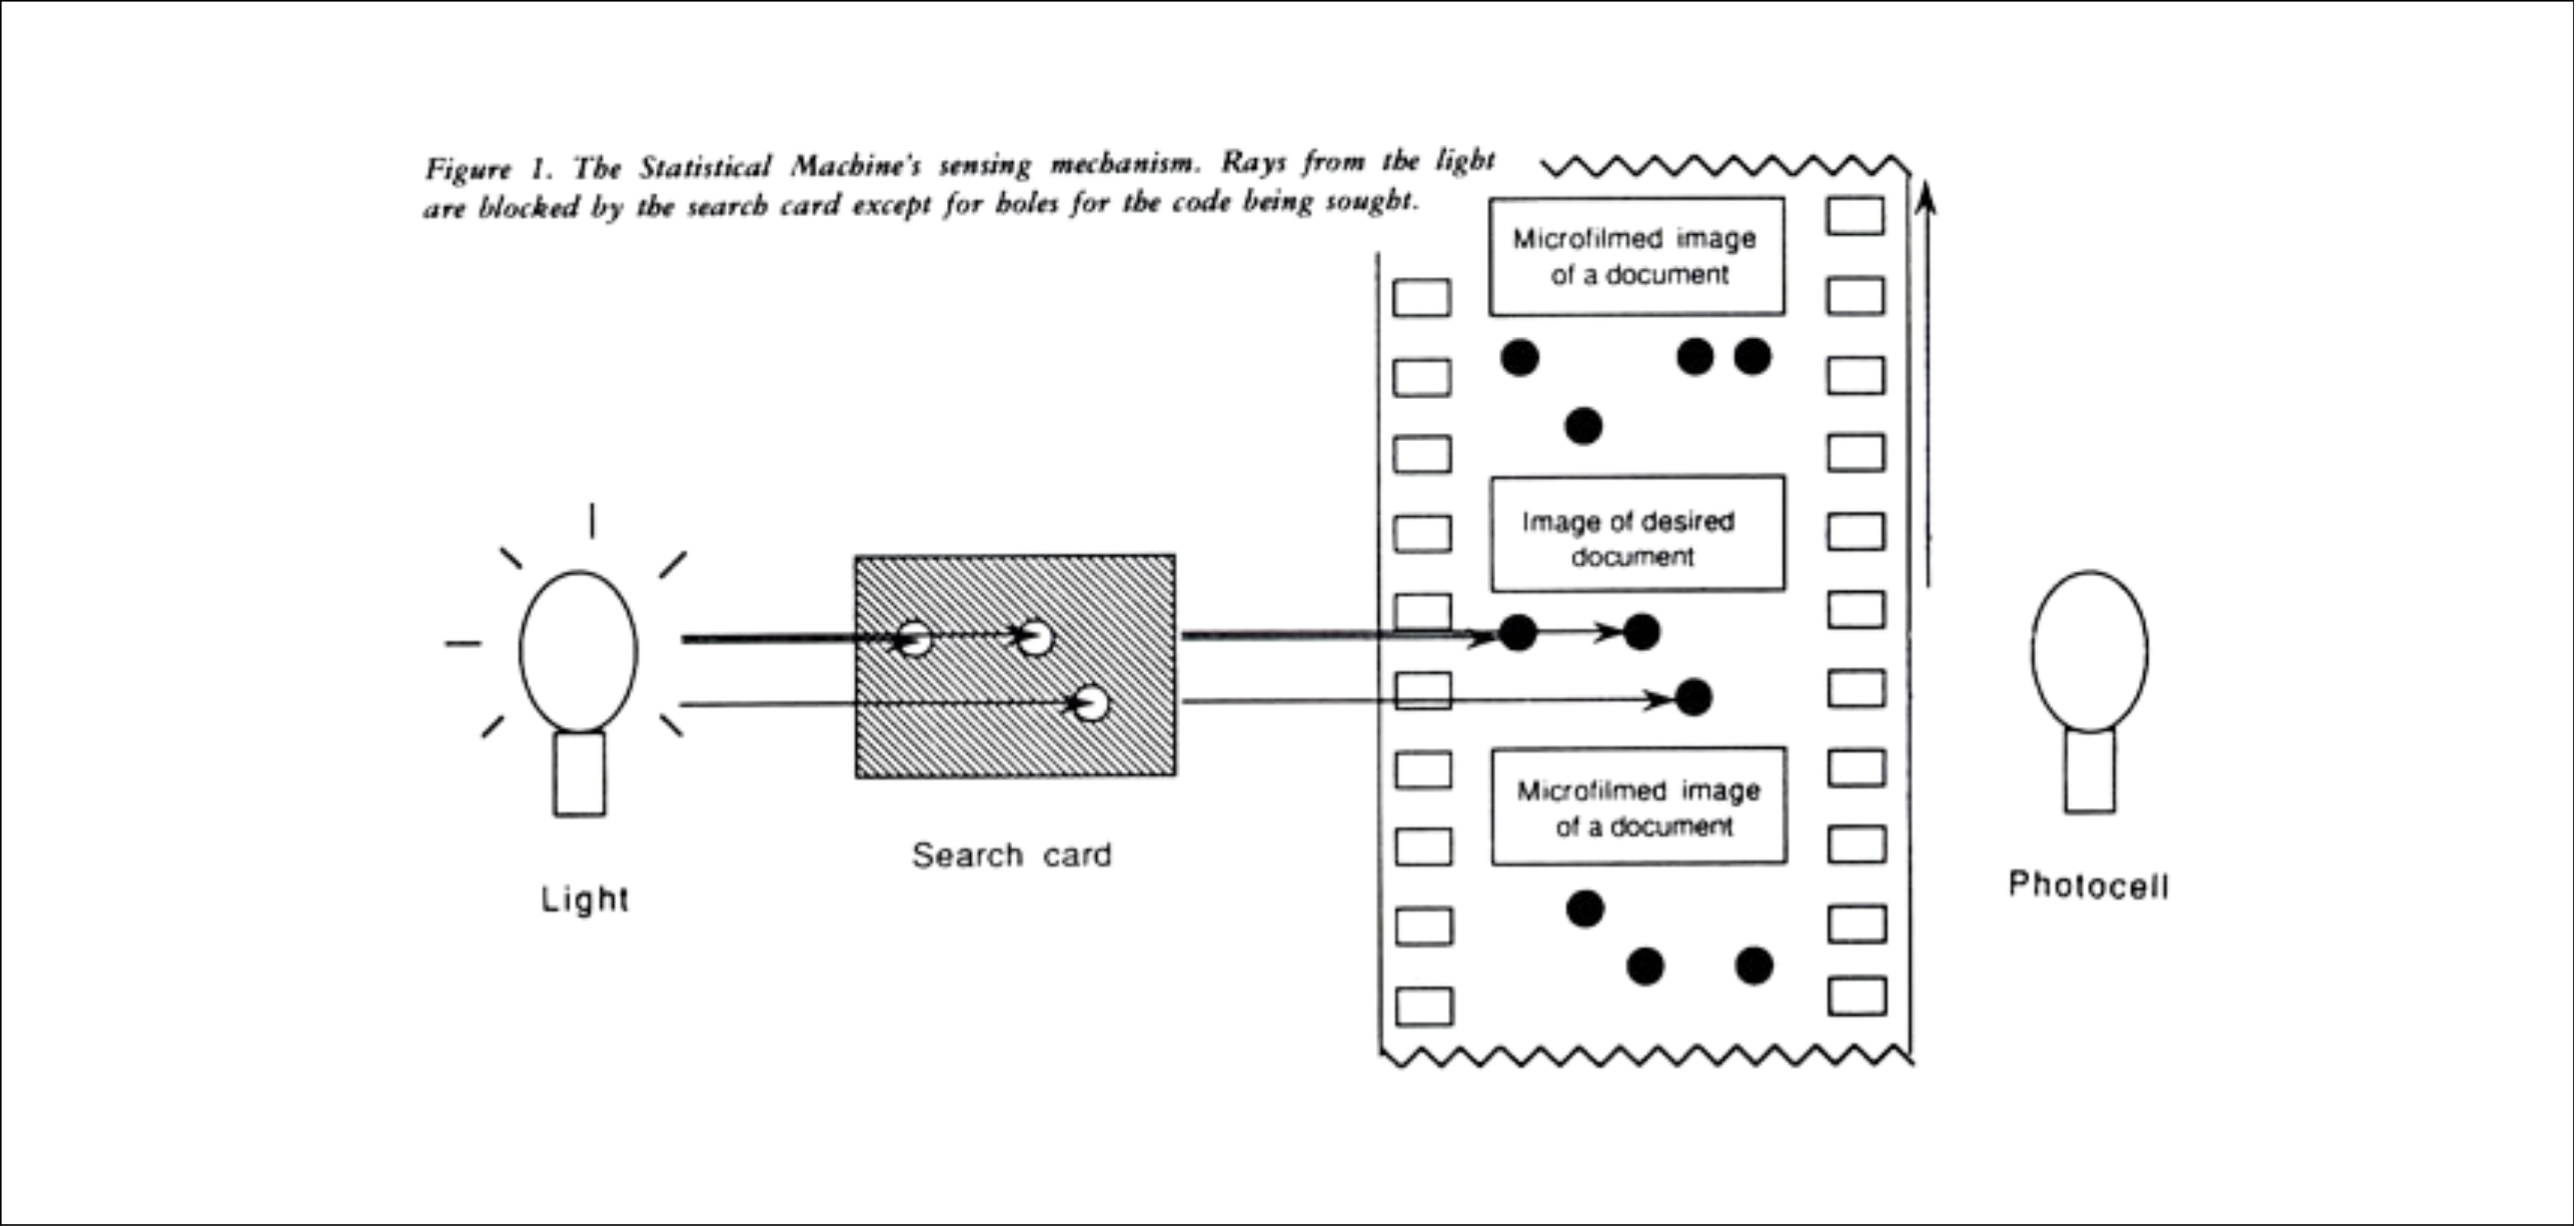
\includegraphics[width=1\textwidth]{figures/statistical_machine_diagram.png}
    \caption{Diagram of Emanuel Goldberg's Statistical Machine (1920s)}
    \label{fig:statistical-machine}
\end{figure}

\subsection{Analog Reading Machine (1930s)}
\phantomsection
\label{sec:analog-reading}

In 1929, Gustav Tauschek, a self-taught Austrian inventor, built upon Goldberg's pioneering work
by adapting the photoelectric detector concept to create his innovative Analog Reading Machine. 
This mechanical marvel represented a significant advancement in early optical character recognition
technology, demonstrating the potential for automated text recognition systems \cite{diem2010recognizing}.

The Reading Machine featured a sophisticated scanning mechanism with a small viewing window designed
to capture text images. As documents passed through this window, an ingeniously designed 
rotating disk system would engage. This disk, meticulously crafted with precise cutouts 
representing various numbers and alphabetic characters, served as the machine's template matching system,
a concept that would later influence modern pattern recognition approaches \cite{diem2010recognizing}.

The operation was remarkably elegant: when the scanned text matched one of the disk's cutout patterns, 
the machine would automatically activate its printing mechanism. A synchronized printing drum would 
then imprint the corresponding characters onto paper, effectively translating visual text into printed 
output. This mechanical automation represented one of the earliest examples of automated text 
recognition and reproduction, laying important groundwork for future OCR developments.

While limited by today's standards, Tauschek's invention demonstrated remarkable ingenuity 
in mechanical pattern recognition and automated text processing. The machine could process 
approximately 80 characters per minute, a significant achievement for its time, though it was 
primarily limited to recognizing printed text in specific fonts and formats, highlighting the 
challenges of character recognition that persist in modern OCR systems \cite{diem2010recognizing}.

\begin{figure}[ht]
    \centering
    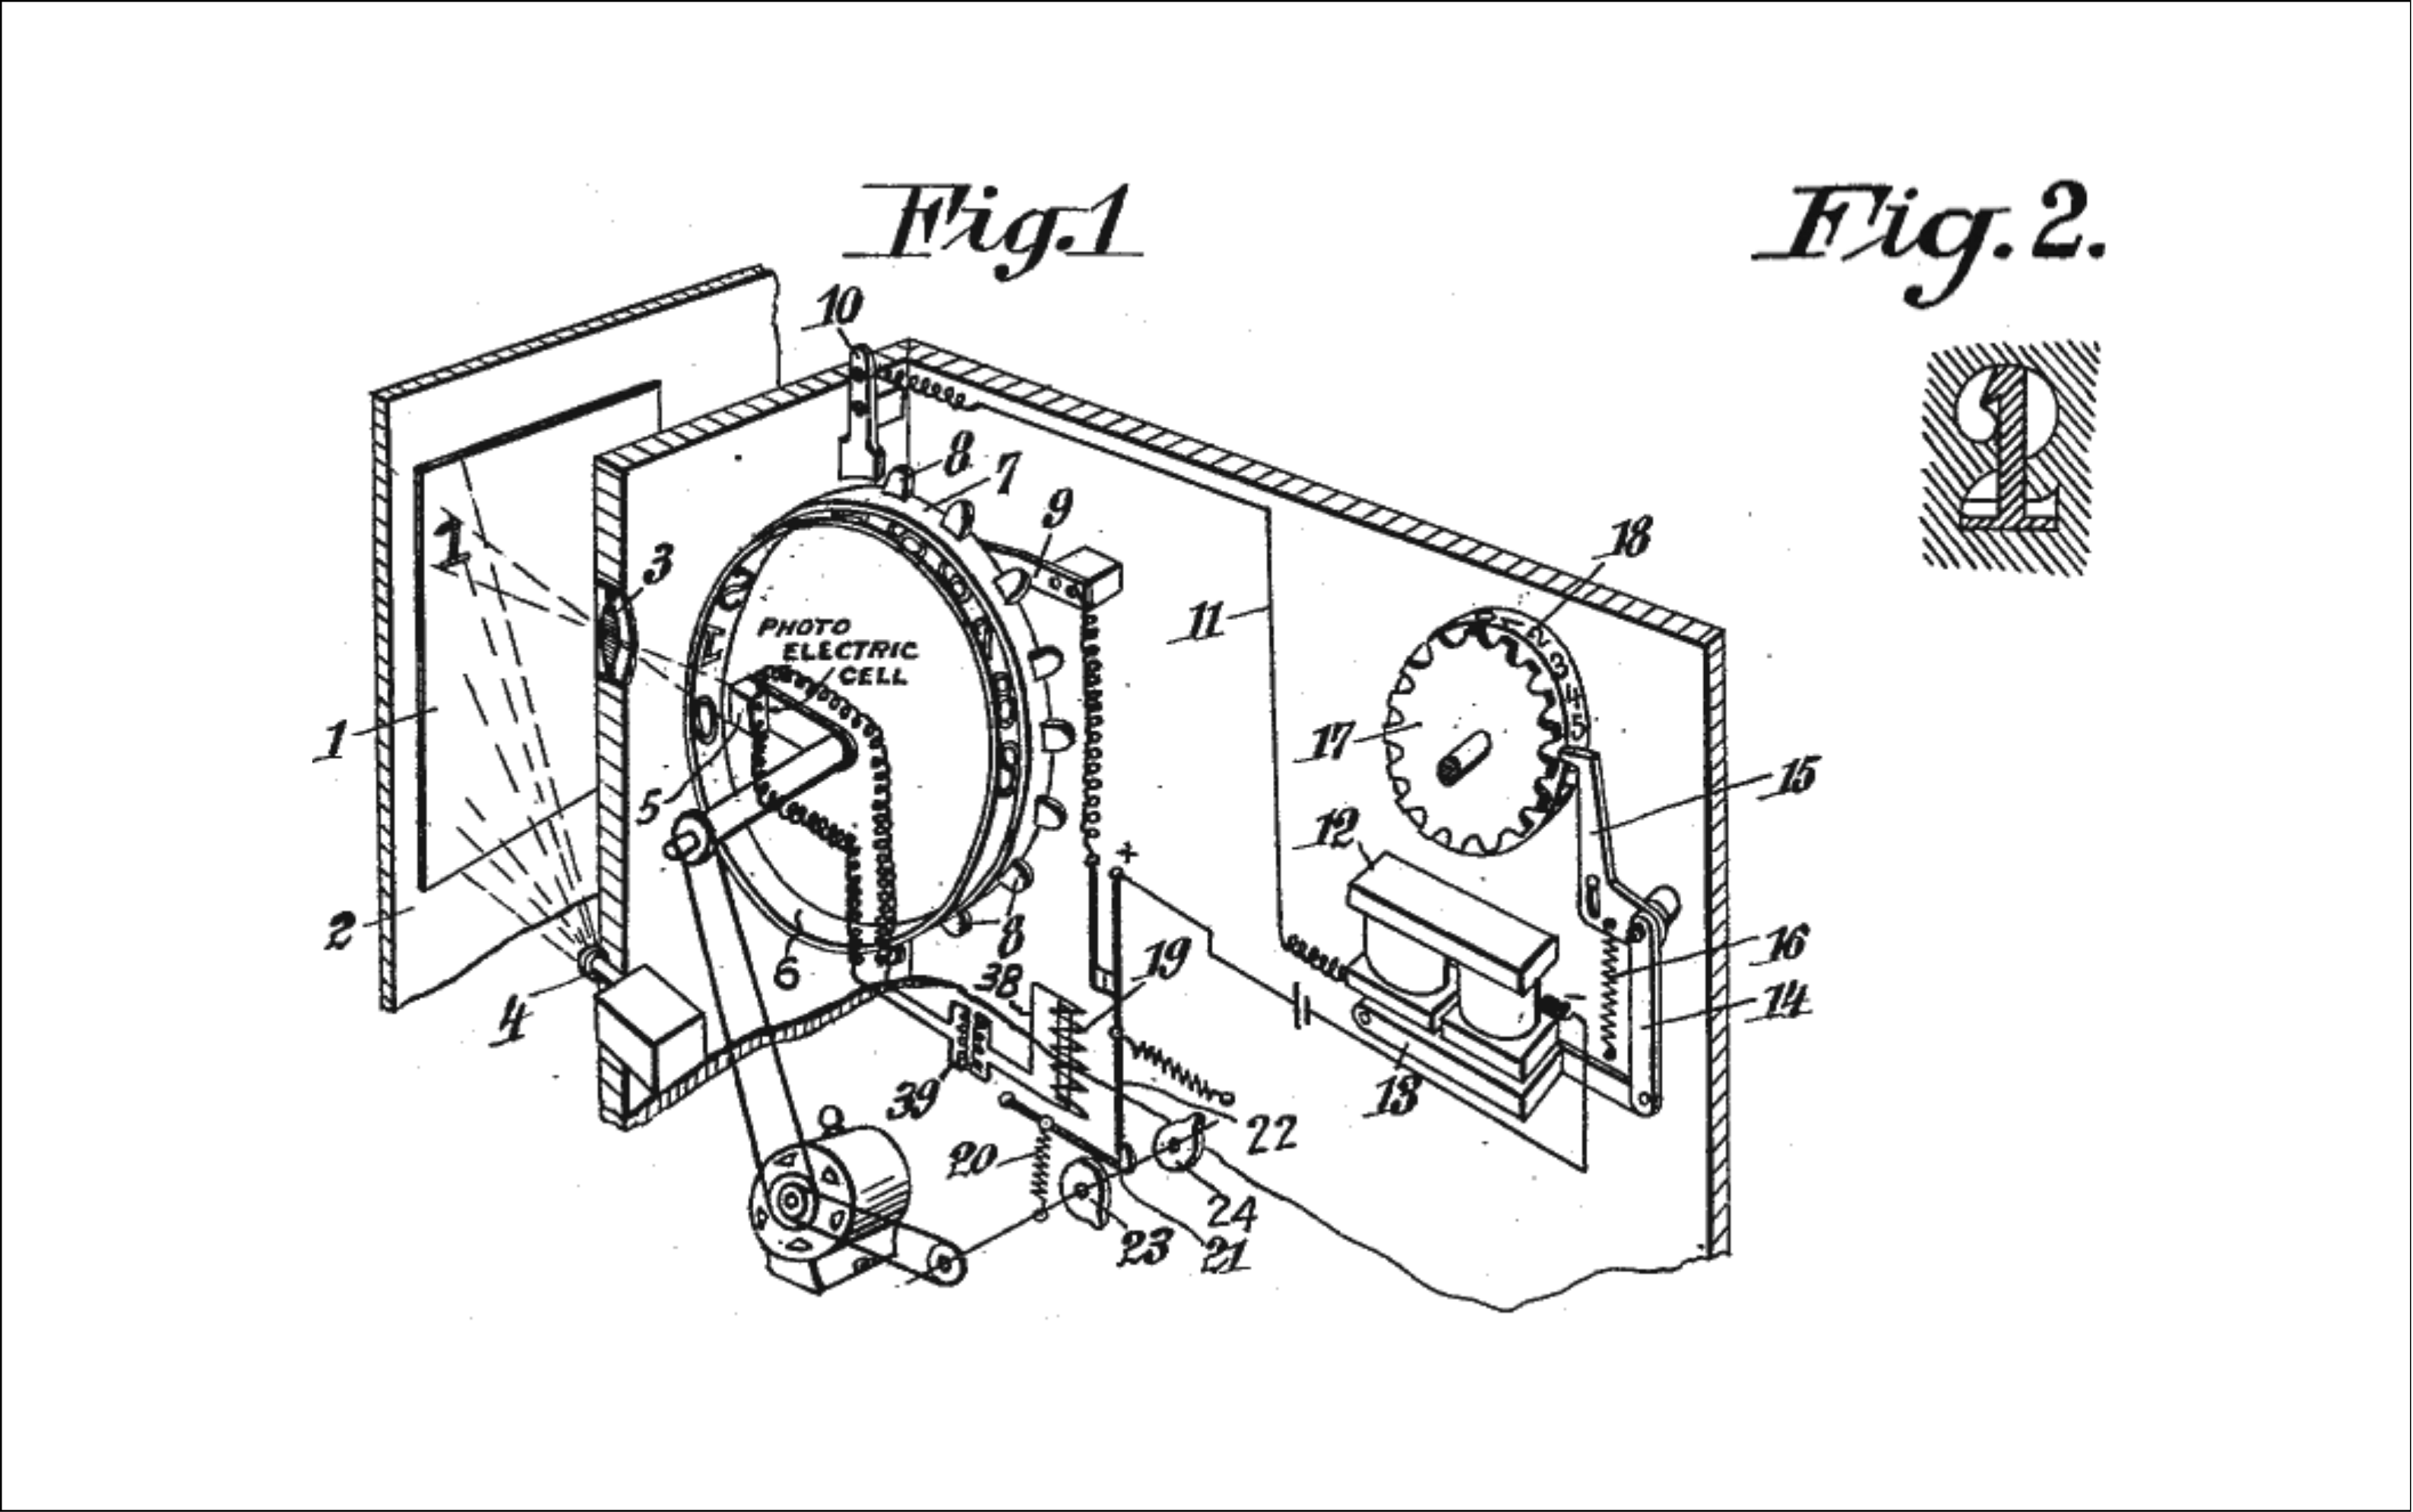
\includegraphics[width=1\textwidth]{figures/Analog_Reading_Machine.png}
    \caption{Tauschek's Analog Reading Machine (1930s) \cite{diem2010recognizing}}
    \label{fig:analog-reading}
\end{figure}


\subsection{First OCR Machine (1950s)}
\phantomsection
\label{sec:first-ocr}

The 1950s were a transformative decade in the history of technology. 
As industries began to generate and rely on increasingly large volumes of data, 
the demand for efficient and automated data processing systems grew significantly. 
Traditional reading machines at the time were limited—they could scan physical 
documents but lacked the ability to translate printed text into digital, machine-readable 
formats. This limitation posed a major challenge to organizations seeking to automate 
information management.

To address this issue, several innovators contributed groundbreaking ideas. Among them 
were David H. Shepard and Harvey Cook Jr., who developed one of the earliest optical character 
recognition (OCR) machines. Their invention, \cite{shepard1953gismo} known as GISMO, was a pioneering solution 
designed to interpret printed characters and convert them into computer-readable code. 
During the patent application process, it was referred to as the "Analyzing Reader."

GISMO represented a significant leap forward in automated data capture. Unlike earlier systems, 
it was capable of recognizing text visually and encoding it into a digital format—a 
foundational step toward the OCR systems we use today. This innovation played a crucial 
role in launching the field of document digitization and information automation, paving 
the way for modern advancements in machine reading and artificial intelligence.

\begin{figure}[ht]
    \centering
    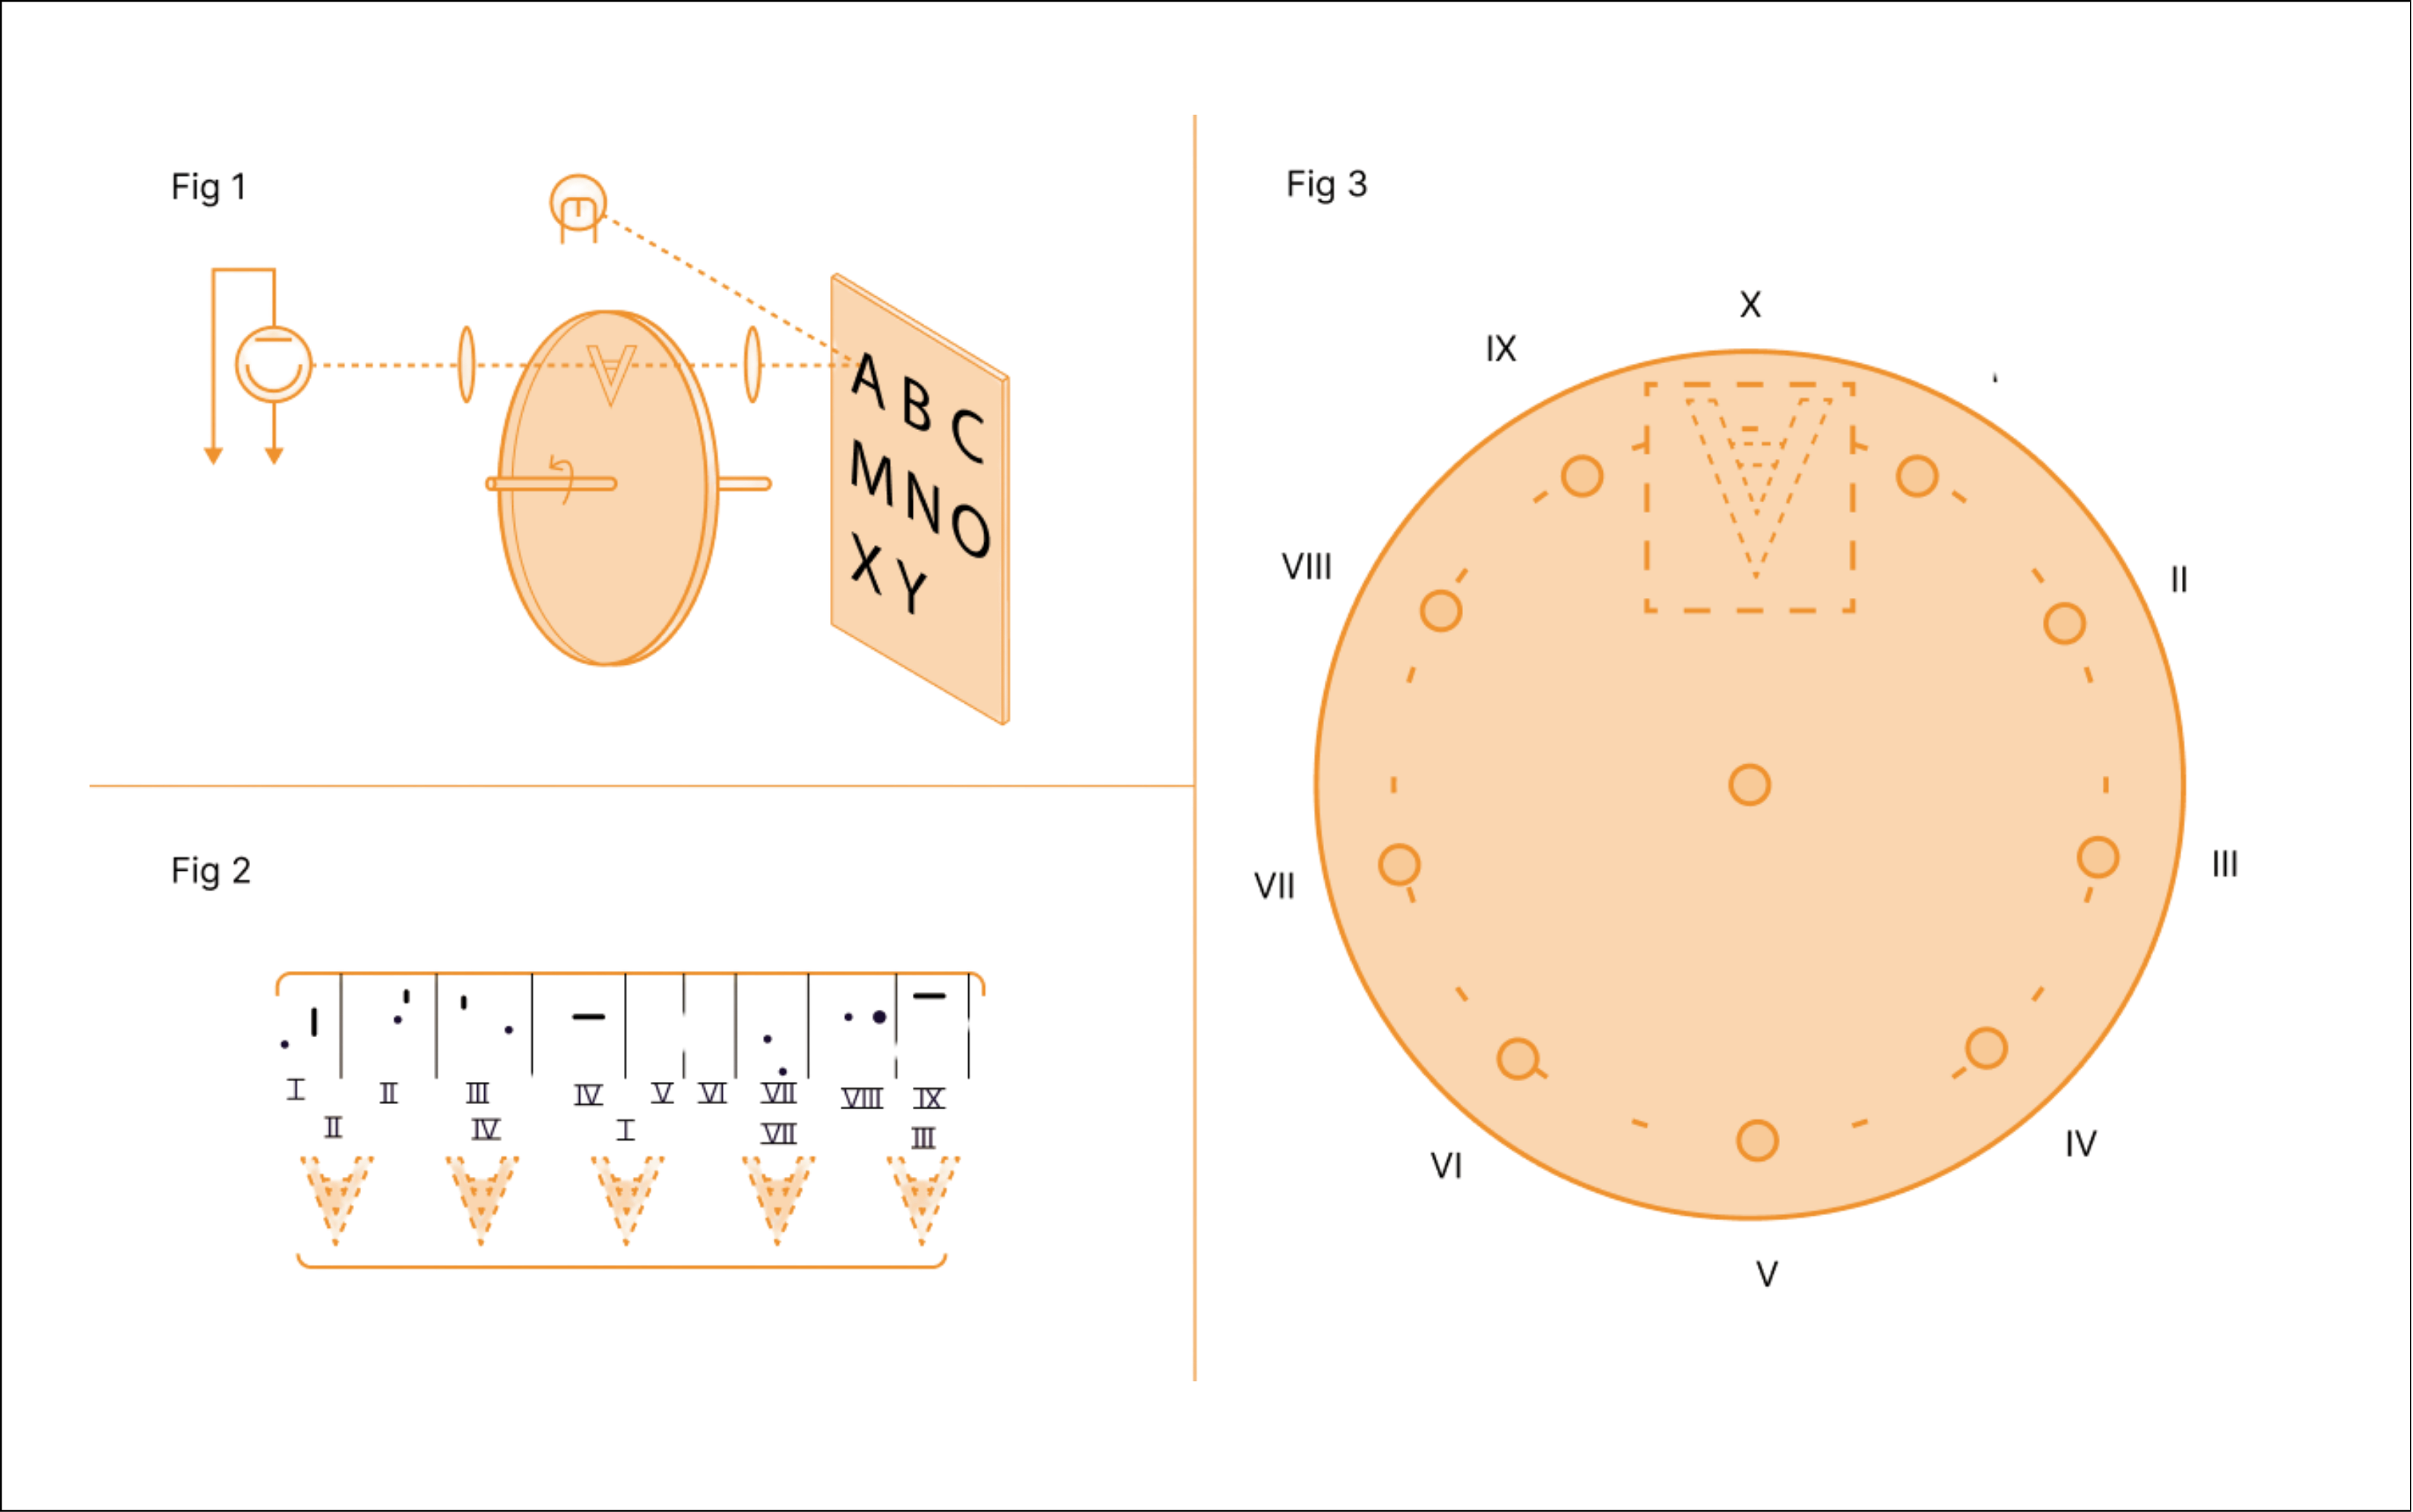
\includegraphics[width=1\textwidth]{figures/David_Shepard_ocr.png}
    \caption{David Shepard's GISMO - The First OCR Machine (1950s) \cite{docsumo2023ocr}}
    \label{fig:shepard-ocr}
\end{figure}

\subsection{Pattern Recognition Advancements (1960s-1970s)}
\phantomsection
\label{sec:pattern-recognition}

In the 1960s, researchers at the Massachusetts Institute of Technology (MIT)  
began working on ways to improve early Optical Character Recognition (OCR) systems. 
Their main goal was to create software that could adapt to different types of documents, 
such as those with various layouts, fonts, and print qualities. They wanted the OCR systems 
to be more flexible and intelligent in how they interpreted scanned text. However, 
the technology at that time had serious limitations. The computers were slow and had 
very little memory, making it difficult to run advanced algorithms. As a result, although 
the researchers had innovative ideas, they couldn't fully implement or test them. These 
efforts, however, laid the foundation for what would later become machine learning in 
OCR — where systems can actually learn and improve over time by processing large amounts of data.

Around the same time, researchers Richard Duda and Peter Hart introduced a powerful new method 
called the Hough Transform \cite{duda1972use}. This algorithm was designed to detect simple 
geometric shapes, such as lines and circles, within images. In the context of OCR, 
this meant machines could now identify the structure of documents — for example, 
where lines of text began and ended, or where printed shapes like logos or seals were located. 
This was a big step forward because it helped OCR systems better understand how to separate 
and process the contents of a page.


Despite its strengths, the Hough Transform also had its downsides. It required a lot of 
computing power and could be sensitive to image noise or low-quality scans. In addition, 
it was designed mainly for detecting basic shapes, not for understanding or recognizing 
complex characters or handwritten text.

In comparison to modern OCR technology, today’s systems use deep learning models like 
convolutional neural networks (CNNs) and transformers (e.g., TrOCR), which can automatically 
detect and recognize characters without needing explicit shape-detection steps. These modern 
systems are much faster, more accurate, and can handle noisy or complex documents far better 
than the early methods like the Hough Transform. Still, the foundational ideas from the 
1960s — including adaptive algorithms and shape detection — played an important role in 
getting us to where we are now. 

\begin{figure}[ht]
    \centering
    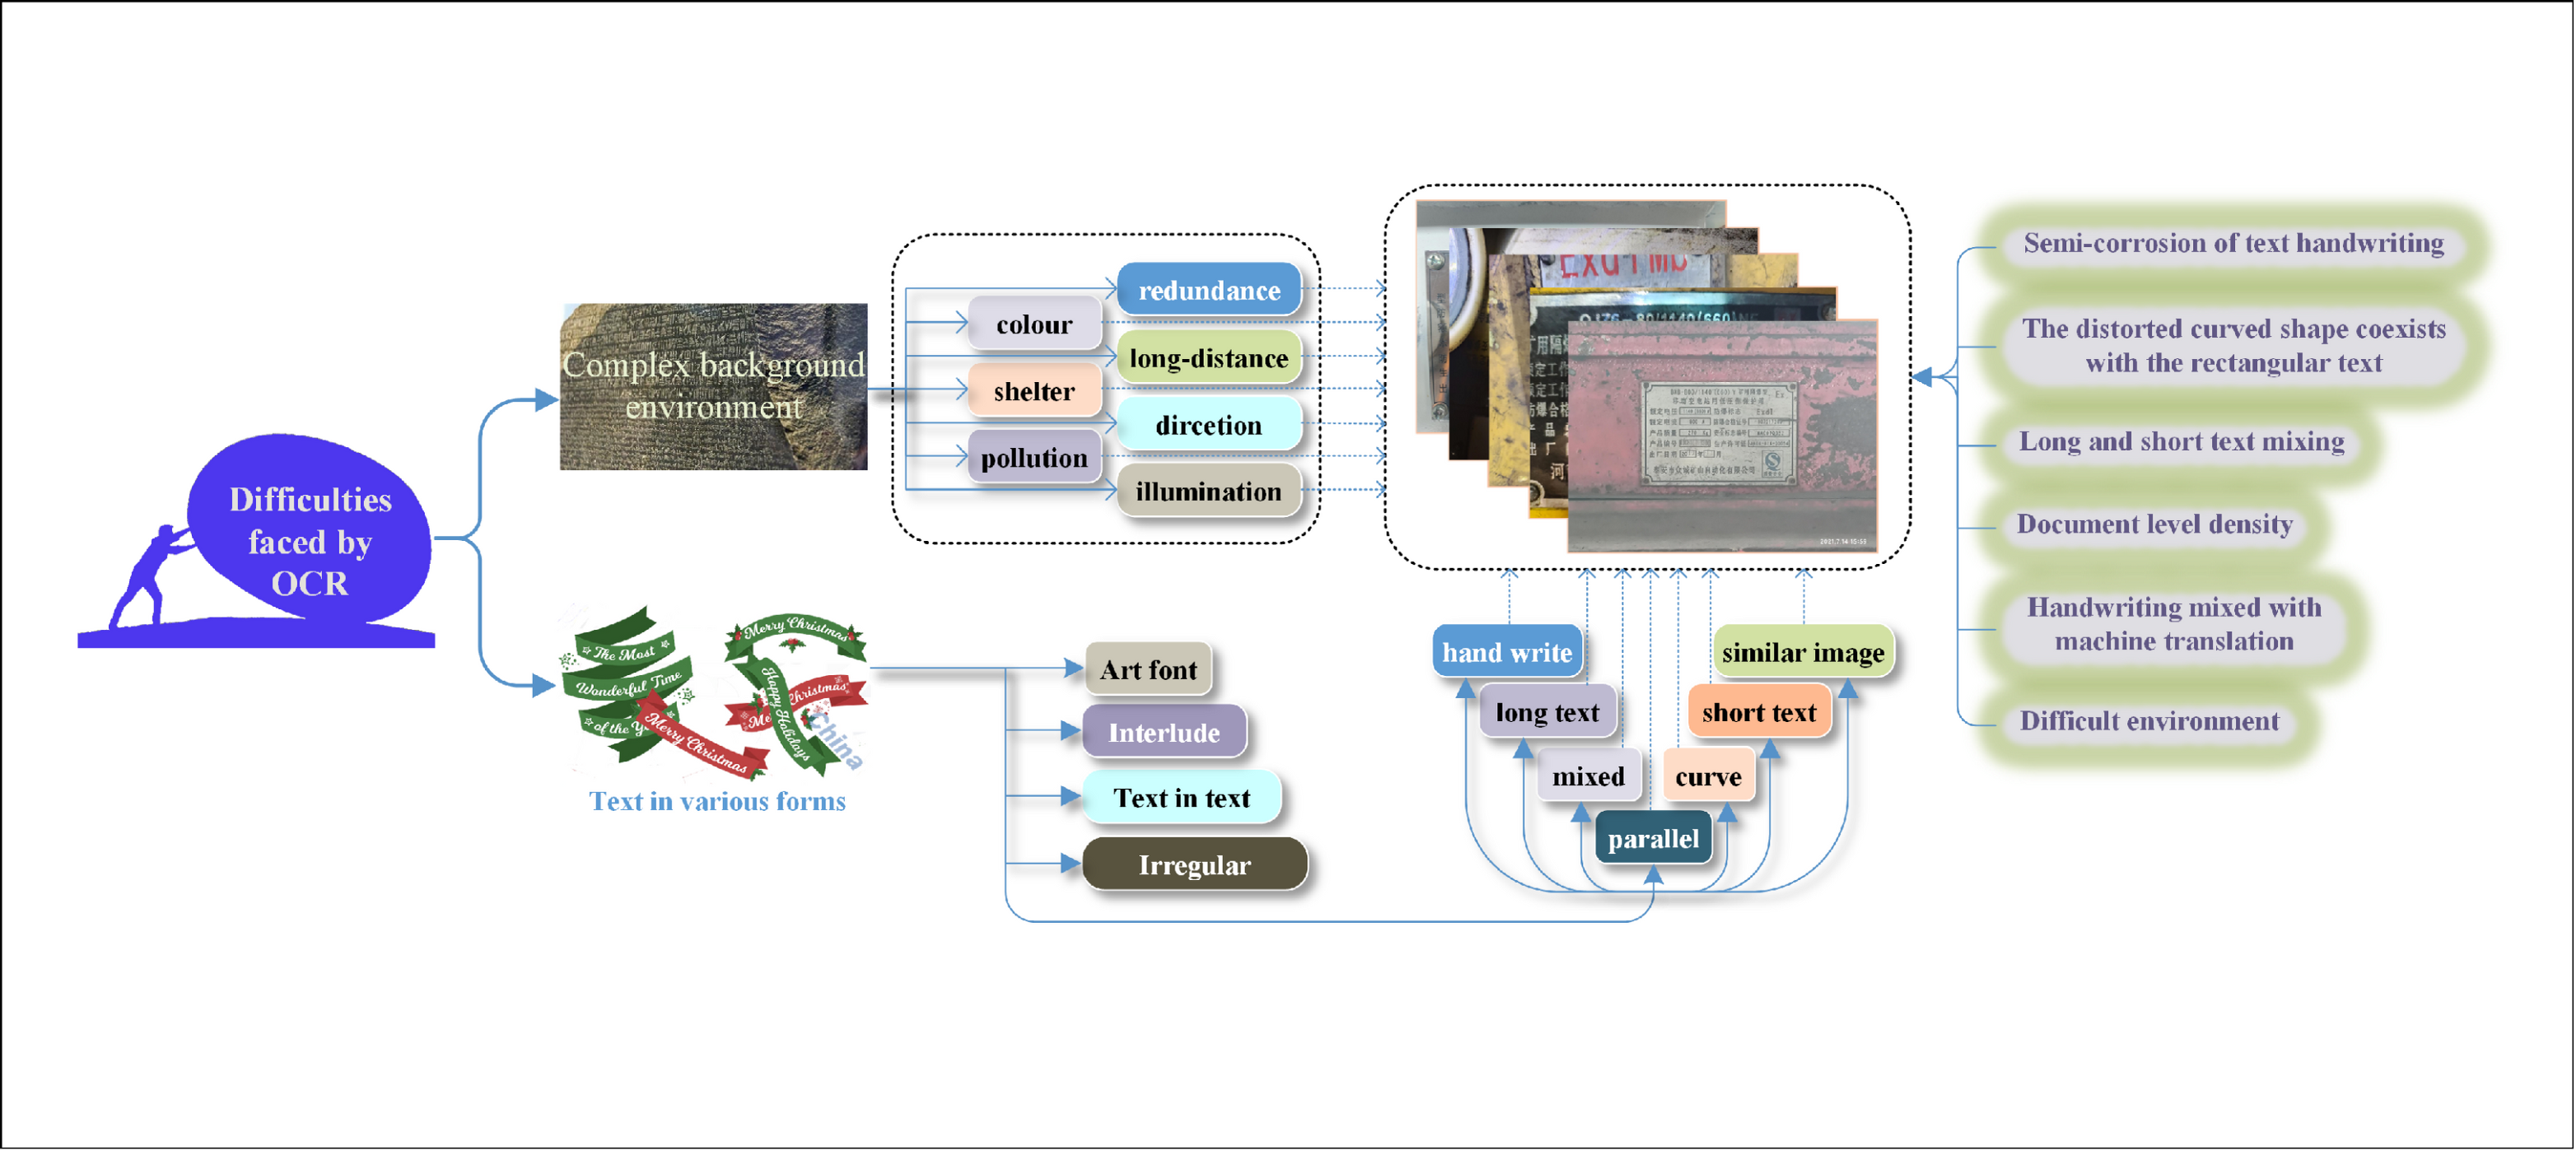
\includegraphics[width=1\textwidth]{figures/Hough_Transform_technique.png}
    \caption{Illustration of the Hough Transform technique developed in the 1960s, 
    which enabled OCR systems to detect geometric features such as lines and circles 
    within scanned documents. This method enhanced document layout analysis and text 
    line segmentation, forming a foundational step in the evolution of 
    structure-aware text detection \cite{liu2023hough}.}
    \label{fig:hough-transform}
\end{figure}


\section{Challenges in Khmer OCR}
\phantomsection
\label{sec:datasets}
A comprehensive review of existing OCR datasets and evaluation benchmarks is presented, with particular focus on those relevant to Southeast Asian scripts and low-resource languages. The limitations of current datasets are also discussed.

\section{Role of Synthetic Data}
\phantomsection
\label{sec:dl-models}

\section{Summary of Research Gaps }
\phantomsection
\label{sec:cnn}
This subsection examines the application of Convolutional Neural Networks in OCR, including architectures specifically designed for text recognition tasks and their performance characteristics.
